\documentclass[border=10pt]{standalone}

\usepackage{tikz}
\usepackage{xcolor}
\usepackage{amsmath}
\usepackage{amssymb}
\usepackage[T1]{fontenc}
\usepackage{helvet}
\renewcommand{\familydefault}{\sfdefault}

\usetikzlibrary{shapes.geometric, arrows.meta, positioning, backgrounds, calc}

%% ── Colours
\definecolor{colDSbdr}{HTML}{334155}   \definecolor{colDSbg}{HTML}{1E293B}
\definecolor{colDSfg} {HTML}{F1F5F9}

\definecolor{colS1bdr}{HTML}{3B82F6}   \definecolor{colS1bg}{HTML}{EFF6FF}
\definecolor{colS1txt}{HTML}{1D4ED8}   \definecolor{colS1sub}{HTML}{DBEAFE}

\definecolor{colPbdr} {HTML}{F59E0B}   \definecolor{colPbg}{HTML}{FFF7ED}
\definecolor{colPtxt} {HTML}{92400E}   \definecolor{colPbdg}{HTML}{B45309}
\definecolor{colPfbg} {HTML}{FEF3C7}

\definecolor{colS2bdr}{HTML}{7C3AED}   \definecolor{colS2bg}{HTML}{F5F3FF}
\definecolor{colS2txt}{HTML}{5B21B6}   \definecolor{colS2sub}{HTML}{EDE9FE}

\definecolor{colLbdr} {HTML}{10B981}   \definecolor{colLbg}{HTML}{ECFDF5}
\definecolor{colLtxt} {HTML}{064E3B}

\definecolor{colMbdr} {HTML}{22C55E}   \definecolor{colMbg}{HTML}{D1FAE5}
\definecolor{colMtxt} {HTML}{14532D}

\definecolor{colGray} {HTML}{94A3B8}
\definecolor{colStxt} {HTML}{6B7280}
\definecolor{colCanvas}{HTML}{F7F8FA}

%% ── Styles
\tikzset{
	blockDS/.style={draw=colDSbdr,fill=colDSbg,rounded corners=6pt,line width=1.8pt,inner sep=9pt},
	blockS1/.style={draw=colS1bdr,fill=colS1bg,rounded corners=6pt,line width=2pt,inner sep=10pt},
	blockP/.style ={draw=colPbdr, fill=colPbg, rounded corners=6pt,line width=2pt,inner sep=10pt},
	blockS2/.style={draw=colS2bdr,fill=colS2bg,rounded corners=6pt,line width=2pt,inner sep=10pt},
	blockL/.style ={draw=colLbdr, fill=colLbg, rounded corners=6pt,line width=2pt,inner sep=10pt},
	blockM/.style ={draw=colMbdr, fill=colMbg, rounded corners=6pt,line width=2pt,inner sep=10pt},
	pillS1/.style={draw=none,fill=colS1bdr,rounded corners=8pt,
		inner xsep=8pt,inner ysep=3pt,
		font=\fontsize{6.5}{7.5}\selectfont\bfseries\sffamily,text=white},
	pillP/.style ={draw=none,fill=colPbdr,rounded corners=8pt,
		inner xsep=8pt,inner ysep=3pt,
		font=\fontsize{6.5}{7.5}\selectfont\bfseries\sffamily,text=white},
	pillS2/.style={draw=none,fill=colS2bdr,rounded corners=8pt,
		inner xsep=8pt,inner ysep=3pt,
		font=\fontsize{6.5}{7.5}\selectfont\bfseries\sffamily,text=white},
	pillL/.style ={draw=none,fill=colLbdr,rounded corners=8pt,
		inner xsep=8pt,inner ysep=3pt,
		font=\fontsize{6.5}{7.5}\selectfont\bfseries\sffamily,text=white},
	pillM/.style ={draw=none,fill=colMbdr,rounded corners=8pt,
		inner xsep=8pt,inner ysep=3pt,
		font=\fontsize{6.5}{7.5}\selectfont\bfseries\sffamily,text=white},
	myArr/.style ={-{Stealth[length=7pt,width=5pt]},line width=1.6pt,color=#1}
}

%% ── Helper: sub-block inside stage panels
%% usage: \subblock{border}{bg}{content}
\newcommand{\subblockSone}[1]{%
	\begin{tikzpicture}
		\node[draw=colS1bdr,fill=colS1sub,rounded corners=4pt,
		line width=1pt,inner sep=8pt,text width=10.2cm]{#1};
\end{tikzpicture}}

\newcommand{\subblockStwo}[1]{%
	\begin{tikzpicture}
		\node[draw=colS2bdr,fill=colS2sub,rounded corners=4pt,
		line width=1pt,inner sep=8pt,text width=10.2cm]{#1};
\end{tikzpicture}}

\newcommand{\resblockSone}[1]{%
	\begin{tikzpicture}
		\node[draw=colS1bdr,fill=colS1bg,dashed,rounded corners=4pt,
		line width=1.2pt,inner sep=8pt,text width=10.2cm]{#1};
\end{tikzpicture}}

\newcommand{\resblockStwo}[1]{%
	\begin{tikzpicture}
		\node[draw=colS2bdr,fill=colS2bg,dashed,rounded corners=4pt,
		line width=1.2pt,inner sep=8pt,text width=10.2cm]{#1};
\end{tikzpicture}}


\begin{document}
	\begin{tikzpicture}[
		font=\sffamily,
		every node/.style={align=center},
		background rectangle/.style={fill=colCanvas},
		show background rectangle
		]
		
		%% ══ TITLE ════════════════════════════════════════════════════
		\node (title) at (0,0) {%
			\begin{minipage}{14cm}\centering
				{\fontsize{13}{15}\selectfont\bfseries
					GNLPDA --- Genetic Nonlinear Linear Discriminant Analysis}\\[4pt]
				{\fontsize{8}{9}\selectfont\color{colStxt}
					HIERARCHICAL FEATURE SELECTION ARCHITECTURE}
		\end{minipage}};
		
		%% ══ DATASET ══════════════════════════════════════════════════
		\node[blockDS, text width=8.5cm, below=14mm of title] (dataset) {%
			{\color{colDSfg}\fontsize{7.5}{9}\selectfont\bfseries INPUT DATASET}\\[4pt]
			{\color{colDSfg}\fontsize{10.5}{12}\selectfont\bfseries
				$N$ samples $\;\cdot\;$ $p$ original features $\;\cdot\;$ $K$ classes}};
		
		%% ══ STAGE 1 ══════════════════════════════════════════════════
		\node[blockS1, text width=11.5cm, below=28mm of dataset] (s1) {%
			\subblockSone{%
				{\color{colS1txt}\fontsize{7}{8}\selectfont\bfseries CHROMOSOME ENCODING}\\[3pt]
				{\fontsize{9.5}{11}\selectfont\color{colS1txt}
					Binary vector $\mathbf{b}\in\{0,1\}^{p}$
					\quad ($b_i=1 \;\Rightarrow\;$ feature $x_i$ selected)}}%
			\\[6pt]
			\subblockSone{%
				{\color{colS1txt}\fontsize{7}{8}\selectfont\bfseries FITNESS FUNCTION}\\[3pt]
				{\fontsize{9.5}{11}\selectfont\color{colS1txt}
					LDA $+$ $k$-fold cross-validation}\\[4pt]
				\colorbox{white}{%
					\fontsize{8.5}{10}\selectfont\ttfamily\color{colS1txt}
					\;fitness = CV-Accuracy(LDA)\;}}%
			\\[6pt]
			\resblockSone{%
				{\fontsize{9.5}{11}\selectfont\color{colS1txt}
					\textbf{Output:} reduced subset of $m$ original variables
					\quad ($m \ll p$)}\\[2pt]
				{\fontsize{9.5}{11}\selectfont\color{colS1txt}
					$x_1,\; x_2,\; \ldots,\; x_m$}}};
		
		\node[pillS1, above=0pt of s1.north]
		{STAGE 1 --- GENETIC SELECTION OF ORIGINAL VARIABLES};
		
		%% ══ POLYNOMIAL EXPANSION ═════════════════════════════════════
		\node[blockP, text width=10.5cm, below=28mm of s1] (poly) {%
			{\color{colPbdg}\fontsize{7}{8}\selectfont\bfseries
				TRANSFORMATION $\;\cdot\;$ BRIDGE BETWEEN STAGES}\\[5pt]
			{\color{colPtxt}\fontsize{12}{14}\selectfont\bfseries
				Restricted Polynomial Expansion (degree~2)}\\[4pt]
			{\color{colPbdg}\fontsize{9.5}{11}\selectfont
				Applied \textit{only} to the $m$ variables selected in Stage~1}\\[6pt]
			\colorbox{colPfbg}{%
				\;\fontsize{9.5}{11}\selectfont\ttfamily\color{colPtxt}
				$\Phi(\mathbf{x}) = \bigl\{\; x_i,\; x_i x_j,\; x_i^{2}
				\;\bigr\}$ \quad for selected $i,\,j$\;}\\[5pt]
			{\color{colPbdg}\fontsize{8.5}{10}\selectfont
				Expanded dimensionality:
				$\;|\Phi| = m + \binom{m}{2} + m$}};
		
		\node[pillP, above=0pt of poly.north]
		{RESTRICTED POLYNOMIAL EXPANSION};
		
		%% ══ STAGE 2 ══════════════════════════════════════════════════
		\node[blockS2, text width=11.5cm, below=28mm of poly] (s2) {%
			\subblockStwo{%
				{\color{colS2txt}\fontsize{7}{8}\selectfont\bfseries CHROMOSOME ENCODING}\\[3pt]
				{\fontsize{9.5}{11}\selectfont\color{colS2txt}
					Binary vector $\mathbf{c}\in\{0,1\}^{|\Phi|}$
					\quad ($c_k=1 \;\Rightarrow\;$ term $\phi_k$ selected)}}%
			\\[6pt]
			\subblockStwo{%
				{\color{colS2txt}\fontsize{7}{8}\selectfont\bfseries FITNESS FUNCTION}\\[3pt]
				{\fontsize{9.5}{11}\selectfont\color{colS2txt}
					LDA $+$ $k$-fold cross-validation}\\[4pt]
				\colorbox{white}{%
					\fontsize{8.5}{10}\selectfont\ttfamily\color{colS2txt}
					\;fitness = CV-Accuracy(LDA)\;}}%
			\\[6pt]
			\resblockStwo{%
				{\fontsize{9.5}{11}\selectfont\color{colS2txt}
					\textbf{Output:} optimal polynomial subspace $\Phi^{*}$}\\[2pt]
				{\fontsize{9.5}{11}\selectfont\color{colS2txt}
					\{selected linear $+$ interaction $+$ quadratic terms\}}}};
		
		\node[pillS2, above=0pt of s2.north]
		{STAGE 2 --- GENETIC SELECTION OF POLYNOMIAL TERMS};
		
		%% ══ LDA CLASSIFIER ═══════════════════════════════════════════
		\node[blockL, text width=10.5cm, below=28mm of s2] (lda) {%
			{\color{colLtxt}\fontsize{7}{8}\selectfont\bfseries
				FINAL CLASSIFIER $\;\cdot\;$ STAGE 3}\\[5pt]
			{\color{colLtxt}\fontsize{12}{14}\selectfont\bfseries
				LDA Classifier Training}\\[4pt]
			{\color{colLtxt}\fontsize{9.5}{11}\selectfont
				Trained on optimal polynomial subspace $\Phi^{*}$}\\[2pt]
			{\color{colLtxt}\fontsize{9.5}{11}\selectfont
				Fisher's linear discriminant criterion
				$\;\cdot\;$ full training set}};
		
		\node[pillL, above=0pt of lda.north]
		{LDA CLASSIFIER};
		
		%% ══ METRICS ══════════════════════════════════════════════════
		\node[blockM, text width=11.5cm, below=26mm of lda] (met) {%
			{\color{colMtxt}\fontsize{7}{8}\selectfont\bfseries EVALUATION OUTPUT}\\[5pt]
			{\color{colMtxt}\fontsize{12}{14}\selectfont\bfseries
				Classification Performance Metrics}\\[8pt]
			\begin{tikzpicture}
				\foreach \m/\x in
				{Accuracy/0, Precision/2.5, Recall/5.0, F1-score/7.5, MCC/10.0}{
					\node[draw=colLbdr,fill=white,rounded corners=3pt,line width=1pt,
					inner sep=5pt,
					font=\fontsize{9}{10}\selectfont\bfseries\ttfamily,
					text=colMtxt] at (\x,0) {\m};}
		\end{tikzpicture}};
		
		\node[pillM, above=0pt of met.north]
		{PERFORMANCE METRICS};
		
		%% ══ ARROWS ═══════════════════════════════════════════════════
		\draw[myArr=colS1bdr] (dataset.south) -- (s1.north);
		
		\draw[myArr=colPbdr] (s1.south) --
		node[right,xshift=5pt,font=\fontsize{8}{9}\selectfont\sffamily,
		text=colPbdg,align=left]
		{only $m$ selected\\variables pass}
		(poly.north);
		
		\draw[myArr=colS2bdr] (poly.south) --
		node[right,xshift=5pt,font=\fontsize{8}{9}\selectfont\sffamily,
		text=colS2txt,align=left]
		{expanded space $\Phi$\\feeds Stage 2}
		(s2.north);
		
		\draw[myArr=colLbdr] (s2.south) --
		node[right,xshift=5pt,font=\fontsize{8}{9}\selectfont\sffamily,
		text=colLtxt]
		{optimal subspace $\Phi^{*}$}
		(lda.north);
		
		\draw[myArr=colLbdr] (lda.south) -- (met.north);
		
		%% ══ LEGEND ═══════════════════════════════════════════════════
		\node[draw=colGray,fill=white,rounded corners=5pt,
		line width=0.8pt,inner sep=10pt,
		below=18mm of met] (legend) {%
			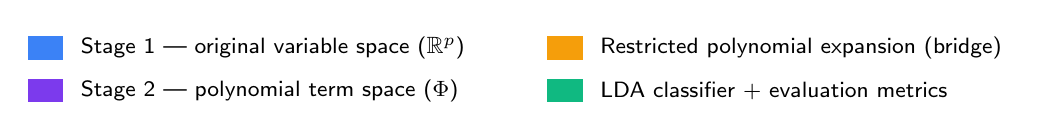
\begin{tikzpicture}[font=\fontsize{8.5}{10}\selectfont\sffamily]
				\fill[colS1bdr] (0,0.04)  rectangle (0.45,0.34);
				\node[right] at (0.55,0.19)
				{Stage 1 --- original variable space ($\mathbb{R}^{p}$)};
				\fill[colPbdr] (6.6,0.04) rectangle (7.05,0.34);
				\node[right] at (7.15,0.19)
				{Restricted polynomial expansion (bridge)};
				\fill[colS2bdr] (0,-0.50) rectangle (0.45,-0.20);
				\node[right] at (0.55,-0.35)
				{Stage 2 --- polynomial term space ($\Phi$)};
				\fill[colLbdr] (6.6,-0.50) rectangle (7.05,-0.20);
				\node[right] at (7.15,-0.35)
				{LDA classifier $+$ evaluation metrics};
		\end{tikzpicture}};
		
	\end{tikzpicture}
\end{document}